\documentclass[tikz, border=10pt]{standalone}
\usepackage{amsmath,amssymb}
\usetikzlibrary{arrows.meta}

\begin{document}

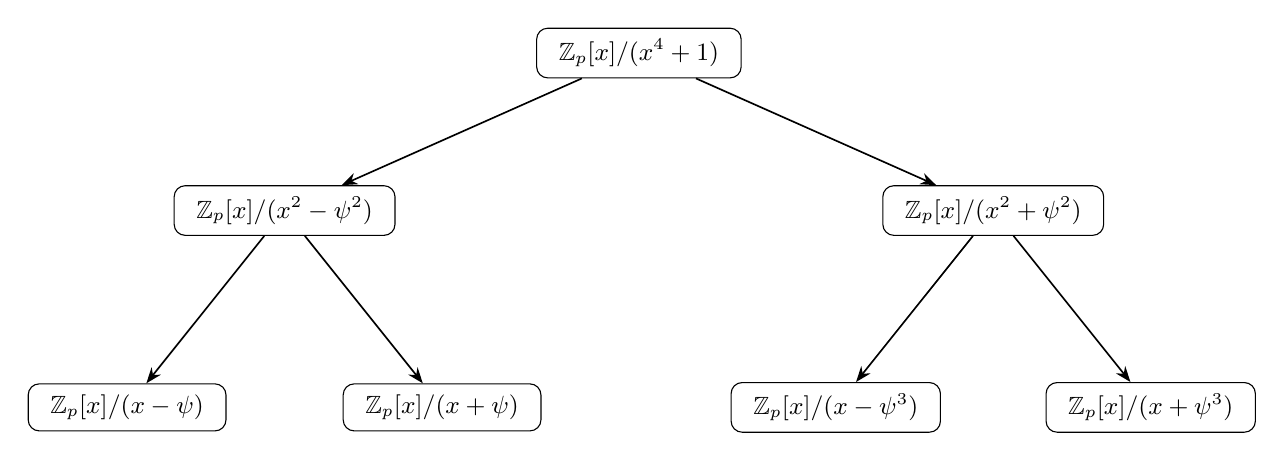
\begin{tikzpicture}[>=Stealth, font=\small]

\tikzset{
  box/.style={draw, rounded corners, align=center, inner xsep=8pt, inner ysep=4pt},
  arr/.style={->, line width=0.6pt}
}

% --- Nós (Coordenadas ajustadas para N=4) ---

% Raiz: N=4
\node[box] (root) at (0,0) {$\mathbb{Z}_p[x]/(x^{4}+1)$};

% Nível 1: Decomposição em grau 2 (N/2 = 2)
% x^4 + 1 = (x^2 - \psi^2)(x^2 + \psi^2)
\node[box] (L1) at (-4.5,-2.0) {$\mathbb{Z}_p[x]/(x^{2}-\psi^{2})$};
\node[box] (R1) at ( 4.5,-2.0) {$\mathbb{Z}_p[x]/(x^{2}+\psi^{2})$};

% Nível 2 (Final): Decomposição em grau 1 (N/4 = 1)

% Lado Esquerdo: Fatores de x^2 - \psi^2
% (x - \psi)(x + \psi)
\node[box] (L2a) at (-6.5,-4.5) {$\mathbb{Z}_p[x]/(x-\psi)$};
\node[box] (L2b) at (-2.5,-4.5) {$\mathbb{Z}_p[x]/(x+\psi)$};

% Lado Direito: Fatores de x^2 + \psi^2
% Sabendo que x^2 + \psi^2 = x^2 - \psi^6 = (x - \psi^3)(x + \psi^3)
% (Note: \psi^6 = -\psi^2 pois \psi^4 = -1)
\node[box] (R2a) at ( 2.5,-4.5) {$\mathbb{Z}_p[x]/(x-\psi^{3})$};
\node[box] (R2b) at ( 6.5,-4.5) {$\mathbb{Z}_p[x]/(x+\psi^{3})$};


% --- Setas ---
% Conexões da Raiz para o Nível 1
\draw[arr] (root) -- (L1);
\draw[arr] (root) -- (R1);

% Conexões do Nível 1 para o Nível Final
\draw[arr] (L1) -- (L2a);
\draw[arr] (L1) -- (L2b);

\draw[arr] (R1) -- (R2a);
\draw[arr] (R1) -- (R2b);

\end{tikzpicture}

\end{document}